%%%%%%%%%%%%%%%%%%%%%%%%%%%%%%%%%%%%%%%%%
% Masters/Doctoral Thesis 
% LaTeX Template
% Version 2.1 (2/9/15)
%
% This template has been downloaded from:
% http://www.LaTeXTemplates.com
%
% Version 2.0 major modifications by:
% Vel (vel@latextemplates.com)
%
% Original authors:
% Steven Gunn  (http://users.ecs.soton.ac.uk/srg/softwaretools/document/templates/)
% Sunil Patel (http://www.sunilpatel.co.uk/thesis-template/)
%
% License:
% CC BY-NC-SA 3.0 (http://creativecommons.org/licenses/by-nc-sa/3.0/)
%
%%%%%%%%%%%%%%%%%%%%%%%%%%%%%%%%%%%%%%%%%

%----------------------------------------------------------------------------------------
%	PACKAGES AND OTHER DOCUMENT CONFIGURATIONS
%----------------------------------------------------------------------------------------

\documentclass[
11pt, % The default document font size, options: 10pt, 11pt, 12pt
%oneside, % Two side (alternating margins) for binding by default, uncomment to switch to one side
english, % ngerman for German
singlespacing, % Single line spacing, alternatives: onehalfspacing or doublespacing
%draft, % Uncomment to enable draft mode (no pictures, no links, overfull hboxes indicated)
%nolistspacing, % If the document is onehalfspacing or doublespacing, uncomment this to set spacing in lists to single
%liststotoc, % Uncomment to add the list of figures/tables/etc to the table of contents
%toctotoc, % Uncomment to add the main table of contents to the table of contents
%parskip, % Uncomment to add space between paragraphs
]{MastersDoctoralThesis} % The class file specifying the document structure

\usepackage[utf8]{inputenc} % Required for inputting international characters
\usepackage[T1]{fontenc} % Output font encoding for international characters

\usepackage{palatino} % Use the Palatino font by default
\usepackage{amssymb}

\usepackage[backend=bibtex,style=authoryear,natbib=true]{biblatex} % User the bibtex backend with the authoryear citation style (which resembles APA)

\addbibresource{example.bib} % The filename of the bibliography

\usepackage[autostyle=true]{csquotes} % Required to generate language-dependent quotes in the bibliography



%----------------------------------------------------------------------------------------
%	THESIS INFORMATION
%----------------------------------------------------------------------------------------

\thesistitle{Fast Projection on Birkhoff polytope} % Your thesis title, this is used in the title and abstract, print it elsewhere with \ttitle
\supervisor{Dr. Rolf \textsc{Bardeli}} % Your supervisor's name, this is used in the title page, print it elsewhere with \supname
\examiner{} % Your examiner's name, this is not currently used anywhere in the template, print it elsewhere with \examname
\degree{Masters of Science} % Your degree name, this is used in the title page and abstract, print it elsewhere with \degreename
\author{Mohammad \textsc{Saifullah}} % Your name, this is used in the title page and abstract, print it elsewhere with \authorname
\addresses{} % Your address, this is not currently used anywhere in the template, print it elsewhere with \addressname

\subject{Media Informatics} % Your subject area, this is not currently used anywhere in the template, print it elsewhere with \subjectname
\keywords{} % Keywords for your thesis, this is not currently used anywhere in the template, print it elsewhere with \keywordnames
\university{\href{http://www.rwth-aachen.de}{RWTH Aachen University}} % Your university's name and URL, this is used in the title page and abstract, print it elsewhere with \univname
\department{\href{http://department.university.com}{Fraunhofer IAIS}} % Your department's name and URL, this is used in the title page and abstract, print it elsewhere with \deptname
\group{\href{http://researchgroup.university.com}{Research Group Name}} % Your research group's name and URL, this is used in the title page, print it elsewhere with \groupname
\faculty{\href{http://faculty.university.com}{Faculty Name}} % Your faculty's name and URL, this is used in the title page and abstract, print it elsewhere with \facname

\hypersetup{pdftitle=\ttitle} % Set the PDF's title to your title
\hypersetup{pdfauthor=\authorname} % Set the PDF's author to your name
\hypersetup{pdfkeywords=\keywordnames} % Set the PDF's keywords to your keywords

\begin{document}

\frontmatter % Use roman page numbering style (i, ii, iii, iv...) for the pre-content pages

\pagestyle{plain} % Default to the plain heading style until the thesis style is called for the body content

%----------------------------------------------------------------------------------------
%	TITLE PAGE
%----------------------------------------------------------------------------------------

\begin{titlepage}
\begin{center}

\textsc{\LARGE \univname}\\[1.5cm] % University name
\textsc{\Large Masters Thesis}\\[0.5cm] % Thesis type

\HRule \\[0.4cm] % Horizontal line
{\huge \bfseries \ttitle}\\[0.4cm] % Thesis title
\HRule \\[1.5cm] % Horizontal line
 
\begin{minipage}{0.4\textwidth}
\begin{flushleft} \large
\emph{Author:}\\
\href{http://www.johnsmith.com}{\authorname} % Author name - remove the \href bracket to remove the link
\end{flushleft}
\end{minipage}
\begin{minipage}{0.4\textwidth}
\begin{flushright} \large
\emph{Supervisor:} \\
\href{http://www.jamessmith.com}{\supname} % Supervisor name - remove the \href bracket to remove the link  
\end{flushright}
\end{minipage}\\[3cm]
 
\large \textit{A thesis submitted in fulfilment of the requirements\\ for the degree of \degreename}\\[0.3cm] % University requirement text
\textit{in the}\\[0.4cm]
\groupname\\\deptname\\[2cm] % Research group name and department name
 
{\large \today}\\[4cm] % Date
%\includegraphics{Logo} % University/department logo - uncomment to place it
 
\vfill
\end{center}
\end{titlepage}

%----------------------------------------------------------------------------------------
%	DECLARATION PAGE
%----------------------------------------------------------------------------------------

\begin{declaration}
\addchaptertocentry{\authorshipname}

\noindent I, \authorname, declare that this thesis titled, \enquote{\ttitle} and the work presented in it are my own. I confirm that:

\begin{itemize} 
\item This work was done wholly or mainly while in candidature for a research degree at this University.
\item Where any part of this thesis has previously been submitted for a degree or any other qualification at this University or any other institution, this has been clearly stated.
\item Where I have consulted the published work of others, this is always clearly attributed.
\item Where I have quoted from the work of others, the source is always given. With the exception of such quotations, this thesis is entirely my own work.
\item I have acknowledged all main sources of help.
\item Where the thesis is based on work done by myself jointly with others, I have made clear exactly what was done by others and what I have contributed myself.\\
\end{itemize}
 
\noindent Signed:\\
\rule[0.5em]{25em}{0.5pt} % This prints a line for the signature
 
\noindent Date:\\
\rule[0.5em]{25em}{0.5pt} % This prints a line to write the date
\end{declaration}

\cleardoublepage

%----------------------------------------------------------------------------------------
%	QUOTATION PAGE
%----------------------------------------------------------------------------------------

\vspace*{0.2\textheight}

\noindent\enquote{\itshape Thanks to my solid academic training, today I can write hundreds of words on virtually any topic without possessing a shred of information, which is how I got a good job in journalism.}\bigbreak

\hfill Dave Barry

%----------------------------------------------------------------------------------------
%	ABSTRACT PAGE
%----------------------------------------------------------------------------------------

\begin{abstract}
\addchaptertocentry{\abstractname} % Add the abstract to the table of contents

The Thesis Abstract is written here (and usually kept to just this page). The page is kept centered vertically so can expand into the blank space above the title too\ldots

\end{abstract}

%----------------------------------------------------------------------------------------
%	ACKNOWLEDGEMENTS
%----------------------------------------------------------------------------------------

\begin{acknowledgements}
\addchaptertocentry{\acknowledgementname} % Add the acknowledgements to the table of contents

The acknowledgements and the people to thank go here, don't forget to include your project advisor\ldots

\end{acknowledgements}

%----------------------------------------------------------------------------------------
%	LIST OF CONTENTS/FIGURES/TABLES PAGES
%----------------------------------------------------------------------------------------

\tableofcontents % Prints the main table of contents

\listoffigures % Prints the list of figures

\listoftables % Prints the list of tables

%----------------------------------------------------------------------------------------
%	ABBREVIATIONS
%----------------------------------------------------------------------------------------

\begin{abbreviations}{ll} % Include a list of abbreviations (a table of two columns)

\textbf{LAH} & \textbf{L}ist \textbf{A}bbreviations \textbf{H}ere\\
\textbf{WSF} & \textbf{W}hat (it) \textbf{S}tands \textbf{F}or\\

\end{abbreviations}

%----------------------------------------------------------------------------------------
%	PHYSICAL CONSTANTS/OTHER DEFINITIONS
%----------------------------------------------------------------------------------------

\begin{constants}{lr@{${}={}$}l} % The list of physical constants is a three column table

% The \SI{}{} command is provided by the siunitx package, see its documentation for instructions on how to use it

Speed of Light & $c$ & \SI{2.99792458e8}{\meter\per\second} (exact)\\
%Constant Name & $Symbol$ & $Constant Value$ with units\\

\end{constants}

%----------------------------------------------------------------------------------------
%	SYMBOLS
%----------------------------------------------------------------------------------------

\begin{symbols}{lll} % Include a list of Symbols (a three column table)

$a$ & distance & \si{\meter} \\
$P$ & power & \si{\watt} (\si{\joule\per\second}) \\
%Symbol & Name & Unit \\

\addlinespace % Gap to separate the Roman symbols from the Greek

$\omega$ & angular frequency & \si{\radian} \\

\end{symbols}

%----------------------------------------------------------------------------------------
%	DEDICATION
%----------------------------------------------------------------------------------------

\dedicatory{For/Dedicated to/To my\ldots} 

%----------------------------------------------------------------------------------------
%	THESIS CONTENT - CHAPTERS
%----------------------------------------------------------------------------------------

\mainmatter % Begin numeric (1,2,3...) page numbering

\pagestyle{thesis} % Return the page headers back to the "thesis" style

% Include the chapters of the thesis as separate files from the Chapters folder
% Uncomment the lines as you write the chapters

% Chapter 1

\chapter{Chapter Title Here} % Main chapter title

\label{Chapter1} % For referencing the chapter elsewhere, use \ref{Chapter1} 

%----------------------------------------------------------------------------------------

% Define some commands to keep the formatting separated from the content 
\newcommand{\keyword}[1]{\textbf{#1}}
\newcommand{\tabhead}[1]{\textbf{#1}}
\newcommand{\code}[1]{\texttt{#1}}
\newcommand{\file}[1]{\texttt{\bfseries#1}}
\newcommand{\option}[1]{\texttt{\itshape#1}}

%----------------------------------------------------------------------------------------

\section{Welcome and Thank You}
Welcome to this \LaTeX{} Thesis Template, a beautiful and easy to use template for writing a thesis using the \LaTeX{} typesetting system.

If you are writing a thesis (or will be in the future) and its subject is technical or mathematical (though it doesn't have to be), then creating it in \LaTeX{} is highly recommended as a way to make sure you can just get down to the essential writing without having to worry over formatting or wasting time arguing with your word processor.

\LaTeX{} is easily able to professionally typeset documents that run to hundreds or thousands of pages long. With simple mark-up commands, it automatically sets out the table of contents, margins, page headers and footers and keeps the formatting consistent and beautiful. One of its main strengths is the way it can easily typeset mathematics, even \emph{heavy} mathematics. Even if those equations are the most horribly twisted and most difficult mathematical problems that can only be solved on a super-computer, you can at least count on \LaTeX{} to make them look stunning.

%----------------------------------------------------------------------------------------

\section{Learning \LaTeX{}}

\LaTeX{} is not a \textsc{wysiwyg} (What You See is What You Get) program, unlike word processors such as Microsoft Word or Apple's Pages. Instead, a document written for \LaTeX{} is actually a simple, plain text file that contains \emph{no formatting}. You tell \LaTeX{} how you want the formatting in the finished document by writing in simple commands amongst the text, for example, if I want to use \emph{italic text for emphasis}, I write the \verb|\emph{text}| command and put the text I want in italics in between the curly braces. This means that \LaTeX{} is a \enquote{mark-up} language, very much like HTML.

\subsection{A (not so short) Introduction to \LaTeX{}}

If you are new to \LaTeX{}, there is a very good eBook -- freely available online as a PDF file -- called, \enquote{The Not So Short Introduction to \LaTeX{}}. The book's title is typically shortened to just \emph{lshort}. You can download the latest version (as it is occasionally updated) from here:
\url{http://www.ctan.org/tex-archive/info/lshort/english/lshort.pdf}

It is also available in several other languages. Find yours from the list on this page: \url{http://www.ctan.org/tex-archive/info/lshort/}

It is recommended to take a little time out to learn how to use \LaTeX{} by creating several, small `test' documents, or having a close look at several templates on:\\ 
\url{http://www.LaTeXTemplates.com}\\ 
Making the effort now means you're not stuck learning the system when what you \emph{really} need to be doing is writing your thesis.

\subsection{A Short Math Guide for \LaTeX{}}

If you are writing a technical or mathematical thesis, then you may want to read the document by the AMS (American Mathematical Society) called, \enquote{A Short Math Guide for \LaTeX{}}. It can be found online here:
\url{http://www.ams.org/tex/amslatex.html}
under the \enquote{Additional Documentation} section towards the bottom of the page.

\subsection{Common \LaTeX{} Math Symbols}
There are a multitude of mathematical symbols available for \LaTeX{} and it would take a great effort to learn the commands for them all. The most common ones you are likely to use are shown on this page:
\url{http://www.sunilpatel.co.uk/latex-type/latex-math-symbols/}

You can use this page as a reference or crib sheet, the symbols are rendered as large, high quality images so you can quickly find the \LaTeX{} command for the symbol you need.

\subsection{\LaTeX{} on a Mac}
 
The \LaTeX{} distribution is available for many systems including Windows, Linux and Mac OS X. The package for OS X is called MacTeX and it contains all the applications you need -- bundled together and pre-customised -- for a fully working \LaTeX{} environment and workflow.
 
MacTeX includes a custom dedicated \LaTeX{} editor called TeXShop for writing your `\file{.tex}' files and BibDesk: a program to manage your references and create your bibliography section just as easily as managing songs and creating playlists in iTunes.

%----------------------------------------------------------------------------------------

\section{Getting Started with this Template}

If you are familiar with \LaTeX{}, then you should explore the directory structure of the template and then proceed to place your own information into the \emph{THESIS INFORMATION} block of the \file{main.tex} file. You can then modify the rest of this file to your unique specifications based on your degree/university. Section \ref{FillingFile} on page \pageref{FillingFile} will help you do this. Make sure you also read section \ref{ThesisConventions} about thesis conventions to get the most out of this template.

If you are new to \LaTeX{} it is recommended that you carry on reading through the rest of the information in this document.

Before you begin using this template you should ensure that its style complies with the thesis style guidelines imposed by your institution. In most cases this template style and layout will be suitable. If it is not, it may only require a small change to bring the template in line with your institution's recommendations. These modifications will need to be done on the \file{MastersDoctoralThesis.cls} file.

\subsection{About this Template}

This \LaTeX{} Thesis Template is originally based and created around a \LaTeX{} style file created by Steve R.\ Gunn from the University of Southampton (UK), department of Electronics and Computer Science. You can find his original thesis style file at his site, here:
\url{http://www.ecs.soton.ac.uk/~srg/softwaretools/document/templates/}

Steve's \file{ecsthesis.cls} was then taken by Sunil Patel who modified it by creating a skeleton framework and folder structure to place the thesis files in. The resulting template can be found on Sunil's site here:
\url{http://www.sunilpatel.co.uk/thesis-template}

Sunil's template was made available through \url{http://www.LaTeXTemplates.com} where it was modified many times based on user requests and questions. Version 2.0 and onwards of this template represents a major modification to Sunil's template and is, in fact, hardly recognisable. The work to make version 2.0 possible was carried out by \href{mailto:vel@latextemplates.com}{Vel} and Johannes Böttcher.

%----------------------------------------------------------------------------------------

\section{What this Template Includes}

\subsection{Folders}

This template comes as a single zip file that expands out to several files and folders. The folder names are mostly self-explanatory:

\keyword{Appendices} -- this is the folder where you put the appendices. Each appendix should go into its own separate \file{.tex} file. An example and template are included in the directory.

\keyword{Chapters} -- this is the folder where you put the thesis chapters. A thesis usually has about six chapters, though there is no hard rule on this. Each chapter should go in its own separate \file{.tex} file and they can be split as:
\begin{itemize}
\item Chapter 1: Introduction to the thesis topic
\item Chapter 2: Background information and theory
\item Chapter 3: (Laboratory) experimental setup
\item Chapter 4: Details of experiment 1
\item Chapter 5: Details of experiment 2
\item Chapter 6: Discussion of the experimental results
\item Chapter 7: Conclusion and future directions
\end{itemize}
This chapter layout is specialised for the experimental sciences.

\keyword{Figures} -- this folder contains all figures for the thesis. These are the final images that will go into the thesis document.

\subsection{Files}

Included are also several files, most of them are plain text and you can see their contents in a text editor. After initial compilation, you will see that more auxiliary files are created by \LaTeX{} or BibTeX and which you don't need to delete or worry about:

\keyword{example.bib} -- this is an important file that contains all the bibliographic information and references that you will be citing in the thesis for use with BibTeX. You can write it manually, but there are reference manager programs available that will create and manage it for you. Bibliographies in \LaTeX{} are a large subject and you may need to read about BibTeX before starting with this. Many modern reference managers will allow you to export your references in BibTeX format which greatly eases the amount of work you have to do.

\keyword{MastersDoctoralThesis.cls} -- this is an important file. It is the class file that tells \LaTeX{} how to format the thesis. If you need to change the layout or structure of the thesis, you will likely need to open this file and find the part relevant to what you are trying to do.

\keyword{main.pdf} -- this is your beautifully typeset thesis (in the PDF file format) created by \LaTeX{}. It is supplied in the PDF with the template and after you compile the template you should get an identical version.

\keyword{main.tex} -- this is an important file. This is the file that you tell \LaTeX{} to compile to produce your thesis as a PDF file. It contains the framework and constructs that tell \LaTeX{} how to layout the thesis. It is heavily commented so you can read exactly what each line of code does and why it is there. After you put your own information into the \emph{THESIS INFORMATION} block -- you have now started your thesis!

Files that are \emph{not} included, but are created by \LaTeX{} as auxiliary files include:

\keyword{main.aux} -- this is an auxiliary file generated by \LaTeX{}, if it is deleted \LaTeX{} simply regenerates it when you run the main \file{.tex} file.

\keyword{main.bbl} -- this is an auxiliary file generated by BibTeX, if it is deleted, BibTeX simply regenerates it when you run the `main' file. Whereas the \file{.bib} file contains all the references you have, this \file{.bbl} file contains the references you have actually cited in the thesis and is used to build the bibliography section of the thesis.

\keyword{main.blg} -- this is an auxiliary file generated by BibTeX, if it is deleted BibTeX simply regenerates it when you run the main \file{.tex} file.

\keyword{main.lof} -- this is an auxiliary file generated by \LaTeX{}, if it is deleted \LaTeX{} simply regenerates it when you run the main \file{.tex} file. It tells \LaTeX{} how to build the \emph{List of Figures} section.

\keyword{main.log} -- this is an auxiliary file generated by \LaTeX{}, if it is deleted \LaTeX{} simply regenerates it when you run the main \file{.tex} file. It contains messages from \LaTeX{}, if you receive errors and warnings from \LaTeX{}, they will be in this \file{.log} file.

\keyword{main.lot} -- this is an auxiliary file generated by \LaTeX{}, if it is deleted \LaTeX{} simply regenerates it when you run the main \file{.tex} file. It tells \LaTeX{} how to build the \emph{List of Tables} section.

\keyword{main.out} -- this is an auxiliary file generated by \LaTeX{}, if it is deleted \LaTeX{} simply regenerates it when you run the main \file{.tex} file.

So from this long list, only the files with the \file{.bib}, \file{.cls} and \file{.tex} extensions are the most important ones. The other auxiliary files can be ignored or deleted as \LaTeX{} and BibTeX will regenerate them.

%----------------------------------------------------------------------------------------

\section{Filling in Your Information in the \file{main.tex} File}\label{FillingFile}

You will need to personalise the thesis template and make it your own by filling in your own information. This is done by editing the \file{main.tex} file in a text editor.

Open the file and scroll down to the second large block titled \emph{THESIS INFORMATION} where you can see the entries for \emph{University Name}, \emph{Department Name}, etc \ldots

Fill out the information about yourself, your group and institution. You can also insert web links, if you do, make sure you use the full URL, including the \code{http://} for this. If you don't want these to be linked, simply remove the \verb|\href{url}{name}| and only leave the name.

When you have done this, save the file and recompile \code{main.tex}. All the information you filled in should now be in the PDF, complete with web links. You can now begin your thesis proper!

%----------------------------------------------------------------------------------------

\section{The \code{main.tex} File Explained}

The \file{main.tex} file contains the structure of the thesis. There are plenty of written comments that explain what pages, sections and formatting the \LaTeX{} code is creating. Each major document element is divided into commented blocks with titles in all capitals to make it obvious what the following bit of code is doing. Initially there seems to be a lot of \LaTeX{} code, but this is all formatting, and it has all been taken care of so you don't have to do it.

Begin by checking that your information on the title page is correct. For the thesis declaration, your institution may insist on something different than the text given. If this is the case, just replace what you see with what is required in the \emph{DECLARATION PAGE} block.

Then comes a page which contains a funny quote. You can put your own, or quote your favourite scientist, author, person, and so on. Make sure to put the name of the person who you took the quote from.

Following this is the abstract page which summaries your work in a condensed way and can almost be used as a standalone document to describe what you have done. The text you write will cause the heading to move up so don't worry about running out of space.

Next come the acknowledgements. On this page, write about all the people who you wish to thank (not forgetting parents, partners and your advisor/supervisor).

The contents pages, list of figures and tables are all taken care of for you and do not need to be manually created or edited. The next set of pages are more likely to be optional and can be deleted since they are for a more technical thesis: insert a list of abbreviations you have used in the thesis, then a list of the physical constants and numbers you refer to and finally, a list of mathematical symbols used in any formulae. Making the effort to fill these tables means the reader has a one-stop place to refer to instead of searching the internet and references to try and find out what you meant by certain abbreviations or symbols.

The list of symbols is split into the Roman and Greek alphabets. Whereas the abbreviations and symbols ought to be listed in alphabetical order (and this is \emph{not} done automatically for you) the list of physical constants should be grouped into similar themes.

The next page contains a one line dedication. Who will you dedicate your thesis to?

Finally, there is the block where the chapters are included. Uncomment the lines (delete the \code{\%} character) as you write the chapters. Each chapter should be written in its own file and put into the \emph{Chapters} folder and named \file{Chapter1}, \file{Chapter2}, etc\ldots Similarly for the appendices, uncomment the lines as you need them. Each appendix should go into its own file and placed in the \emph{Appendices} folder.

After the preamble, chapters and appendices finally comes the bibliography. The bibliography style (called \option{authoryear}) is used for the bibliography and is a fully featured style that will even include links to where the referenced paper can be found online. Do not underestimate how grateful your reader will be to find that a reference to a paper is just a click away. Of course, this relies on you putting the URL information into the BibTeX file in the first place.

%----------------------------------------------------------------------------------------

\section{Thesis Features and Conventions}\label{ThesisConventions}

To get the best out of this template, there are a few conventions that you may want to follow.

One of the most important (and most difficult) things to keep track of in such a long document as a thesis is consistency. Using certain conventions and ways of doing things (such as using a Todo list) makes the job easier. Of course, all of these are optional and you can adopt your own method.

\subsection{Printing Format}

This thesis template is designed for double sided printing (i.e. content on the front and back of pages) as most theses are printed and bound this way. This means that the inner margin is always wider than the outer for binding. Four out of five people will now judge the margins by eye and think, \enquote{I never noticed that before}. Switching to one sided printing is as simple as uncommenting the \option{oneside} option of the \code{documentclass} command at the top of the \file{main.tex} file. You may then wish to adjust the margins to suit specifications from your institution.

The headers for the pages contain the page number on the outer side (so it is easy to flick through to the page you want) and the chapter name on the inner side.

The text is set to 11 point by default with single line spacing, again, you can tune the text size and spacing should you want or need to using the options at the very start of \file{main.tex}. The spacing can be changed similarly by replacing the \option{singlespacing} with \option{onehalfspacing} or \option{doublespacing}.

\subsection{Using US Letter Paper}

The paper size used in the template is A4, which is the standard size in Europe. If you are using this thesis template elsewhere and particularly in the United States, then you may have to change the A4 paper size to the US Letter size. To do this, you will need to open the \file{MastersDoctoralThesis.cls} file and navigate to the \code{MARGINS} block where you can change \option{a4paper} to \option{letterpaper}.

Due to the differences in the paper size, the resulting margins may be different to what you like or require (as it is common for institutions to dictate certain margin sizes). If this is the case, then the margin sizes can be tweaked by modifying the values in the same block as where you set the paper size. Now your document should be set up for US Letter paper size with suitable margins.

\subsection{References}

The \code{biblatex} package is used to format the bibliography and inserts references such as this one \parencite{Reference1}. The options used in the \file{main.tex} file mean that the in-text citations of references are formatted with the author(s) listed with the date of the publication. Multiple references are separated by semicolons (e.g. \parencite{Reference2, Reference1}) and references with more than three authors are only show the first author with \emph{et al.} indicating there are more authors (e.g. \parencite{Reference3}). This is done automatically for you. To see how you use references, have a look at the \file{Chapter1.tex} source file. Many reference managers allow you to simply drag the reference into the document as you type.

Scientific references should come \emph{before} the punctuation mark if there is one (such as a comma or period). The same goes for footnotes\footnote{Such as this footnote, here down at the bottom of the page.}. You can change this but the most important thing is to keep the convention consistent throughout the thesis. Footnotes themselves should be full, descriptive sentences (beginning with a capital letter and ending with a full stop). The APA6 states: ``Footnote numbers should be superscripted, [...], following any punctuation mark except a dash.'' The Chicago manual of style states: ``A note number should be placed at the end of a sentence or clause. The number follows any punctuation mark except the dash, which it precedes. It follows a closing parenthesis.''

The bibliography is typeset with references listed in alphabetical order by the first author's last name. This is similar to the APA referencing style. To see how \LaTeX{} typesets the bibliography, have a look at the very end of this document (or just click on the reference number links in in-text citations).

\subsubsection{A Note on bibtex}

The bibtex backend used in the template by default does not correctly handle unicode character encoding (i.e. "international" characters). You may see a warning about this in the compilation log and, if your references contain unicode characters, they may not show up correctly or at all. The solution to this is to use the biber backend instead of the outdated bibtex backend. This is done by finding this in \file{main.tex}: \option{backend=bibtex} and changing it to \option{backend=biber}. You will then need to delete all auxiliary BibTeX files and navigate to the template directory in your terminal (command prompt). Once there, simply type \code{biber main} and biber will compile your bibliography. You can then compile \file{main.tex} as normal and your bibliography will be updated. An alternative is to set up your LaTeX editor to compile with biber instead of bibtex, see \href{http://tex.stackexchange.com/questions/154751/biblatex-with-biber-configuring-my-editor-to-avoid-undefined-citations/}{here} for how to do this for various editors.

\subsection{Tables}

Tables are an important way of displaying your results, below is an example table which was generated with this code:

{\small
\begin{verbatim}
\begin{table}
\caption{The effects of treatments X and Y on the four groups studied.}
\label{tab:treatments}
\centering
\begin{tabular}{l l l}
\toprule
\tabhead{Groups} & \tabhead{Treatment X} & \tabhead{Treatment Y} \\
\midrule
1 & 0.2 & 0.8\\
2 & 0.17 & 0.7\\
3 & 0.24 & 0.75\\
4 & 0.68 & 0.3\\
\bottomrule\\
\end{tabular}
\end{table}
\end{verbatim}
}

\begin{table}
\caption{The effects of treatments X and Y on the four groups studied.}
\label{tab:treatments}
\centering
\begin{tabular}{l l l}
\toprule
\tabhead{Groups} & \tabhead{Treatment X} & \tabhead{Treatment Y} \\
\midrule
1 & 0.2 & 0.8\\
2 & 0.17 & 0.7\\
3 & 0.24 & 0.75\\
4 & 0.68 & 0.3\\
\bottomrule\\
\end{tabular}
\end{table}

You can reference tables with \verb|\ref{<label>}| where the label is defined within the table environment. See \file{Chapter1.tex} for an example of the label and citation (e.g. Table~\ref{tab:treatments}).

\subsection{Figures}

There will hopefully be many figures in your thesis (that should be placed in the \emph{Figures} folder). The way to insert figures into your thesis is to use a code template like this:
\begin{verbatim}
\begin{figure}
\centering

\includegraphics{Figures/Electron}
\decoRule
\caption[An Electron]{An electron (artist's impression).}
\label{fig:Electron}
\end{figure}
\end{verbatim}
Also look in the source file. Putting this code into the source file produces the picture of the electron that you can see in the figure below.

\begin{figure}[h]
\centering

\includegraphics{Figures/Electron}
\decoRule
\caption[An Electron]{An electron (artist's impression).}
\label{fig:Electron}
\end{figure}

Sometimes figures don't always appear where you write them in the source. The placement depends on how much space there is on the page for the figure. Sometimes there is not enough room to fit a figure directly where it should go (in relation to the text) and so \LaTeX{} puts it at the top of the next page. Positioning figures is the job of \LaTeX{} and so you should only worry about making them look good!

Figures usually should have captions just in case you need to refer to them (such as in Figure~\ref{fig:Electron}). The \verb|\caption| command contains two parts, the first part, inside the square brackets is the title that will appear in the \emph{List of Figures}, and so should be short. The second part in the curly brackets should contain the longer and more descriptive caption text.

The \verb|\decoRule| command is optional and simply puts an aesthetic horizontal line below the image. If you do this for one image, do it for all of them.

\LaTeX{} is capable of using images in many formats such as PDF, JPEG, PNG and more.

\subsection{Typesetting mathematics}

If your thesis is going to contain heavy mathematical content, be sure that \LaTeX{} will make it look beautiful, even though it won't be able to solve the equations for you.

The \enquote{Not So Short Introduction to \LaTeX} (available on \href{http://www.ctan.org/tex-archive/info/lshort/english/lshort.pdf}{CTAN}) should tell you everything you need to know for most cases of typesetting mathematics. If you need more information, a much more thorough mathematical guide is available from the AMS called, \enquote{A Short Math Guide to \LaTeX} and can be downloaded from:
\url{ftp://ftp.ams.org/pub/tex/doc/amsmath/short-math-guide.pdf}

There are many different \LaTeX{} symbols to remember, luckily you can find the most common symbols \href{http://www.sunilpatel.co.uk/latexsymbols.html}{here}. You can use the web page as a quick reference or crib sheet and because the symbols are grouped and rendered as high quality images (each with a downloadable PDF), finding the symbol you need is quick and easy.

You can write an equation, which is automatically given an equation number by \LaTeX{} like this:
\begin{verbatim}
\begin{equation}
E = mc^{2}
\label{eqn:Einstein}
\end{equation}
\end{verbatim}

This will produce Einstein's famous energy-matter equivalence equation:
\begin{equation}
E = mc^{2}
\label{eqn:Einstein}
\end{equation}

All equations you write (which are not in the middle of paragraph text) are automatically given equation numbers by \LaTeX{}. If you don't want a particular equation numbered, use the unnumbered form:
\begin{verbatim}
\[ a^{2}=4 \]
\end{verbatim}

%----------------------------------------------------------------------------------------

\section{Sectioning and Subsectioning}

You should break your thesis up into nice, bite-sized sections and subsections. \LaTeX{} automatically builds a table of Contents by looking at all the \verb|\chapter{}|, \verb|\section{}|  and \verb|\subsection{}| commands you write in the source.

The Table of Contents should only list the sections to three (3) levels. A \verb|chapter{}| is level zero (0). A \verb|\section{}| is level one (1) and so a \verb|\subsection{}| is level two (2). In your thesis it is likely that you will even use a \verb|subsubsection{}|, which is level three (3). The depth to which the Table of Contents is formatted is set within \file{MastersDoctoralThesis.cls}.

%----------------------------------------------------------------------------------------

\section{In Closing}

You have reached the end of this mini-guide. You can now rename or overwrite this pdf file and begin writing your own \file{Chapter1.tex}' and the rest of your thesis. The easy work of setting up the structure and framework has been taken care of for you. It's now your job to fill it out!

Good luck and have lots of fun!

\begin{flushright}
Guide written by ---\\
Sunil Patel: \href{http://www.sunilpatel.co.uk}{www.sunilpatel.co.uk}\\
Vel: \href{http://www.LaTeXTemplates.com}{LaTeXTemplates.com}
\end{flushright}
% Chapter Template

\chapter{The Birkhoff Polytope} % Main chapter title

\label{ChapterX} % Change X to a consecutive number; for referencing this chapter elsewhere, use \ref{ChapterX}



%----------------------------------------------------------------------------------------
%	SECTION 1
%----------------------------------------------------------------------------------------
In this Chapter I am going to describe about Birkhoff polytope $B_n$ which is sometimes considered to be one of the most important polytopes in many sphere. Before that I will define some basic types.
\section{Hypermatrix}

A generalisation of matrix to an $n_1 \times n_1 \times ...$ array of numbers. \newline
Example: 3-dimensional hypermatrix(cube). It is a $2 \times 2 \times 2$ matrix over $\mathbb{R}$.


\begin{figure}[h]
\centering
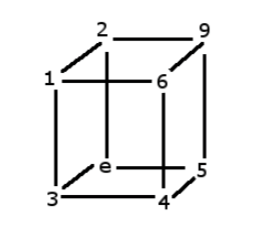
\includegraphics{Figures/hypercube.png}
\decoRule
\caption[hypercube]{3-dimensional hypermatrix(cube).}
\label{fig:hypercube}
\end{figure}

\section{Doubly-Stochastic Matrix}

Doubly Stochastic Matrix is a square matrix of non-negative real numbers, each of whose rows and columns sum to 1. If rows and columns of some matrices sum to n, it can also be considered as doubly stochastic matrix because we can just device all the entries by n, which results to true Doubly Stochastic.\\


Examples:

\[
  \begin{bmatrix}
    0 & 1 & 0 \\
    1 & 0 & 0 \\
    0 & 0 & 1 \\
  \end{bmatrix}
  ,
    \begin{bmatrix}
     1/6 & 5/6 & 0 & 0 \\
     0 & 0 & 1 & 0 \\
     0 & 1/6 & 0 & 5/6 \\
     5/6 & 0 & 0 & 1/6
    \end{bmatrix}
  ,
    \begin{bmatrix}
     \frac{1}{2} & \frac{1}{2} \\
     \frac{1}{2} & \frac{1}{2}
    \end{bmatrix}
\]

\section{Permutation Matrix}

A matrix obtained by permuting the rows of an $n\times n$ identity matrix according to some permutation of the numbers 1 to n. So the number of $n\times n$ permutation matrics is $n!$.\\

The permutation matrics of order 3 are:
\[
  \begin{bmatrix}
    1 & 0 & 0 \\
    0 & 1 & 0 \\
    0 & 0 & 1 \\
  \end{bmatrix}
  ,
    \begin{bmatrix}
     1 & 0 & 0 \\
     0 & 0 & 1 \\
     0 & 1 & 0 \\
    \end{bmatrix}
  ,
    \begin{bmatrix}
     0 & 0 & 1 \\
     1 & 0 & 0 \\
     0 & 1 & 0 \\
    \end{bmatrix}
    ,
    \begin{bmatrix}
     0 & 1 & 0 \\
     1 & 0 & 0 \\
     0 & 0 & 1 \\
    \end{bmatrix}
    ,
    \begin{bmatrix}
     0 & 1 & 0 \\
     0 & 0 & 1 \\
     1 & 0 & 0 \\
    \end{bmatrix}
    ,
    \begin{bmatrix}
     0 & 0 & 1 \\
     0 & 1 & 0 \\
     1 & 0 & 0 \\
    \end{bmatrix}
\]


\section{Polytopes}

In elementary geometry, a polytope is a geometric object with flat sides, and may exist in any general number of dimensions n as an n-dimensional polytope or n-polytope. For example a two-dimensional polygon is a 2-polytope and a three-dimensional polyhedron is a 3-polytope

Mathematically, A polytope $P\subseteq \mathbb{R}^d$ is the convex hull $P=conv(v_1,...,v_k)$ of a finite set of points $v_1,...,v_k \in \mathbb{R}^d$ . Dually any polytope can be written as the bounded intersection of a finite number of affine half-spaces in the form $P = \{ x\mid Ax \leq b \}$

\subsection{Elements of polytope}
A proper face of $F$ of a polytope $P$ is the intersection of $P$ with and affine hyperplane $H$ such that $P$ is completely contained in one of the closed half spaces defined by $H$. The empty set and the polytope P a face of $P$. Any face $F$ is itself  polytope. The dimension of a polytope $P \subseteq \mathbb{R}^d$ is the dimension of the minimum affine space containin it. It is full dimensional if its dimension is d.

0-dimensional faces of $P$ are called $vertices$, 1-dimensional faces are edges. Proper faces of maximal dimensional are called facets. $P$ is the convex hull of its vertices, and the vertices of any face are subset of the vertices of $P$. Thus, a polytope has only a finite number of faces. Let $f_i$ be the number of $i$-dimensional faces of $P,0 \leq i \leq dim P-1$. The $f$-vector of a d-dimensional polytope P is the non-negative integral vector $f(P) = (f_0,...,f_(d-1)$.

The face lettice or combinatorial type $\mathcal{L}(P)$ of a polytope P is the partially ordered set of all faces of P (including the empty face and P itself). This defines Eulerian lattice. Figure shows 2.1 this lattice.


It contains all combinatorial information of the polytope. Two polytopes P,$P'$ are combinatorially isomorphic or have the same combinatorial type if their face lattices are isomorphic as posets.

An r-dimensional simplex (or r-simplex) is the convex hull of r+1 affinely independent points in $\mathbb{R}^d$. A polytope is called simplicial if all facets are simplices. It is simple if the dual is simplicial. Equally, a d-dimensilanl polytope P is simple if each vertex is incident to precisely d edges. The d-dimensional 0/1-cube $C^d$ is the convexhull of all d-dimensinal 0/1-vectors. This is a simple d-polytope with $2^d$ vertices and 2d facets. More generally we denote by a d-cube any d-dimensional polytope that is combinatorially isomorphic to the 0/1-cube (it need not be full dimensional).

\subsection{Properties of Polytope}
Let $P_1 \subset \mathbb{R}^{d_1}$ and $P_2 \subset \mathbb{R}^{d_2}$ be two (geometrically realized) polytopes with vertex sets $V(P_1)=\{ v_1,...,v_k$ and $V(P_2)=\{ w_1,...,w_l \}$. With $0^{(d)}$ we denote he d-dimensional zero vector.

The (geometric) product of $P_1$ and $P_2$ is the polytope

\begin{equation}
P_1 \times P_2 = conv( (v_i,w_i)\in \mathbb{R}^{d_1+d_2}\mid 1\leq i \leq k, i \leq j \leq l)
\label{eqn:Einstein}
\end{equation}

This is the same as the set of all points $(v,w)$ for $v \in P_1$ and $w \in P_2$. The (geometric) join of $P_1$ and $P_2$ is the polytope

\begin{equation}
P_1 \star P_2 := conv(P_1 \times \{ 0^{d_2} \} \times \{ 0 \} \cup \{ 0^{d_1} \} \times P_2 \times \{ 1 \} ) \subseteq \mathbb{R}^{d_1+d_2+1}
\label{eqn:Einstein}
\end{equation}

More generally we say that a polytope P is a product or join of two polytopes $P_1$ and $P_2$, if P is combinatorially isomorphic to the geometric prouct or geometric join of some realisations of the face lattices $P_1$, or $P_2$.

If $F$ is face of a polytope  $P = \{ x \mid Ax \leq b \} \subseteq \mathbb{R}^d$  and $ \langle c,x \rangle \leq d $ a linear funtional defining F, then the $wedge wedge_F(P)$ of P over F is defined to be the polytope.
 
\begin{equation}
wedge_F(P) = \{ (x,x_0) \in \mathbb{R}^{d+1} \mid Ax\leq b, 0\leq x_0 \leq d- \langle c,x \rangle\}
\label{eqn:Einstein}
\end{equation}

Again, we say more generally that P is wedge of a polytope  Q over some face F of Q if P is combinatorially equivalently to $wedge_F(Q)$



%----------------------------------------------------------------------------------------
%	SECTION 2
%----------------------------------------------------------------------------------------

\section{Birkhoff Polytope}

Birkhoff polytope $B_n$ is sometimes considered to be one of the most important polytopes in many sphere. Birkhoff polytope is also called assignment polytope, the polytope of doubly stochastic matrices, or the perfect matching polytope of complete bipartite graph $K_(n,n)$ ,transportation polytope. It surprisingly appears in various branches of mathematics from geometry to enumerative combinatorics to optimisation theory to Statistics.

The Birkhoff polytope $B_n$ is the convex hull of all $(n\times n)$ permutation metrices, i.e.matrices which consists precisely one 1 in every row and column, and zeros at all places. Equivalently, $B_n$ is the set of all non-negative $(n \times n)$-metrices, whose rows and columns all sum to 1, or the perfect matching polytope of the complete bipartite graph $K_(n,n)$. The Birkhoff polytope $B_n$ has dimension $(n-1)^2$ with $n!$ vertices and $n_2$ facets. The Birkhoff-von Neumann Theoram illustrated, $B_n$ can be understood as the intersection of the positive orthant with a family of of hyperplanes.

Birkhoff polytopes are widely studied as a class of polytopes in the area of optimisation, statistics, enumerative combinatorics or representation theory. Despite, Combinatorial and Geometrical structure of Birkhoff polytope and its algorithmic treatment are still open to disover.

A Birkhoff polytope $B_n$ is a polytope defined by the following equations and in-equalities:
\begin{equation}
a_{i,j} \geqslant 0, \sum_{i=1}^{n} a_{i,j} = 1, \sum_{j=1}^{n} a_{i,j}=1 \text{ for all } 1\leqslant i,j\leqslant n.
\label{eqn:Birkhoff_definition}
\end{equation}	

$(a_{i,j}$ can be thought of as  $n\times n$ doubly stochastic matrices. It can be realise that $B_n$ has dimension $(n-1)^2$ as values of $a_{i,j},1\leqslant i,j\leqslant n$ determine the rest. Different way helps to realise that vertices of $P_n$ are permutation matrices.

\section{Properties of $B_n$}
Here I am going to describe some of the properties of Birkhoff polytope.
\subsection{Vetices}
The Birkhoff polytope has $n!$ vertices. This was derived from the Birkhoff-von Neumann theorem.
\subsection{Edges}
The edges of the Birkhoff polytope corresponds to pairs of permutations differing by a cycle:

$(\sigma,\omega)$ such that $\sigma^{-1}\omega$ is a cycle.

This implies that the graph of $B_n$ is a Caley graph of the symmetric group $S_n$. This ialso implies that the graph of $B_3$ is a complete graph $K_6$, and thus $B_3$ is a neighbourly prototype.

\subsection{Facets}
The Birkhoff polytope lies within and $(n^2-2n+1)$-dimensional affine subspace of the $n^2$-dimensional space of all $n\times n$ matrices: this subspace is determined by the linear equality constraints that the sum of each row and each column be one. Within this subspace, it is defined by $n^2$ linear inequalities, one for each coordinate of the matrix, specifying that the coordinate be non-negative. Therefore, it has exactly $n^2$ facets.

\subsection{Symmetries}
The Birkhoff polytop $B_n$ is both vertex-transitive and facet-transitive. This is not regular for $n>2$.

\subsection{Volume}
One of the hardest open problem is to find the volume of a Birkhoff polytopes. Volume calculation was possible for $n\leqslant 10$. It is known to be equal to the volume of polytope associated with standard Young tabuleaux. The following asymptotic formula was founded by Rodney Canifeld and Brenden McKay:

\begin{equation}
vol(B_n)=\exp(-(n-1)^2 \ln n + n^2 - (n-\frac{1}{2} )\ln(2\pi)+\frac{1}{3}+\mathcal{O}(1))
\label{eqn:Birkhoff_volume}
\end{equation}	
% Chapter Template

\chapter{Quadratic Programming} % Main chapter title

\label{ChapterX} % Change X to a consecutive number; for referencing this chapter elsewhere, use \ref{ChapterX}

%----------------------------------------------------------------------------------------
%	SECTION 1
%----------------------------------------------------------------------------------------
An optimisation problem with a quadratic objective function and linear constraints is called a quadratic program. Problem of this type are important in their own right, and they also arise as subproblems in methods for general constrained optimisations. 

\section{Definition of QP}

The general quadratic program(QP) can be stated as

\begin{equation}
\begin{aligned}
& \underset{x}{\text{min}}
& & q(x)= \frac{1}{2}x^{T}Gx+x^{T}c \\
& \text{subject to} & &  a_{i}^{T}x = b_i & i\in \mathbb{E} \\
& & &  a_i^{T}x \geqslant b_{i} & i\in \mathbb{I}
\end{aligned}
\label{eqn:quadratic_programming}
\end{equation}
where $G$ is a symmetric $n\times n$ matrix, $E$ and $I$ are finite sets of indices, and $c$,$x$, and $a_i, i\in E \cup I$, are vectors in $\mathbb{R}^n$. Quadratic programs can always be solved (or shown to be infeasible) in a finite amount of computation, but the effort required to find a solution depends strongly on the characteristics of the objective function and the number of inequality constraints. If the Hessian matrix $G$ is positive semidefinite, we say that \ref{eqn:quadratic_programming} is a convex QP, and in this case the problem is often similar in difficulty to a linear program. (Strictly convex QPs are those in which G is positive definite.) Nonconvex QPs, in which G is an indefinite matrix, can be more challenging because they can have several stationary points and local minima.

In this chapter we will try to show different kinds of quadratic programs but we will mainly focus on convex quadratic program and different algorithms of convex quadratic programs.

\section{Classification of QP's}

Some classification of quadratic program's:
\begin{itemize}
	\item Unconstrianed QP
	\item Box constrained QP
	\item Equality constrained QP
	\item Inequality constrained QP.
\end{itemize}

\section*{Important Definitions}
\subsection*{Logarithmic barrier}
Consider inequalities $Ax \leqslant b$ with $A$ of size $m\times n$ and with rows $a_i^T$
define
\begin{equation*}
P=\lbrace x \mid Ax \leqslantb \rbrace \text{ and } P^0=\lbrace x \mid Ax < b \rbrace
\end{equation*}

\subsection*{KKT System}
KKT System is
\subsection*{Hessian Matrix}
Hessian Matrix is.
\subsection*{Active set}
The Active set $\mathbb{A}(x)$ at any feasible $x$ consists of the equality constraint indices from $\varepsilon$ together with the indices of the inequality constraints $i$ for which $c_i(x)=0$; that is,
\begin{equation*}
	\begin{aligned}
		\mathbb{A}(x)=\varepsilon \cup {i\in \mathbb{I}\mid c_i(x)=0}
	\end{aligned}
\end{equation*}
At a feasible point x, the inequality constraint $i\in \mathbb{I}$ is said to be active if $c_i(x)=0$ and inactive if the strict inequality $c_i(x)>0$ is satisfied.

\section{Equality-Constrained Quadratic Programs}

We start this section with of algorithms for quadratic programming by considering the case of equality constrained

\subsection*{Properties of Equality-constrained QPs}
To make it simple, we write the equality constraint in a form of matrix and define it as follows:

\begin{equation}
\begin{aligned}
& \underset{x}{\text{min}}
& & q(x)= \frac{1}{2}x^{T}Gx+x^{T}c \\
& \text{subject to} & &  Ax=b
\end{aligned}
\label{eqn:equality_constrained_QP}
\end{equation}

where $A$ is the $m\times n$ Jacobian of constraints (with $m\leqslant n$) whose rows are $a_i^T,i \in \mathbb{E}$ and $b$ is the vecotor in $\mathbb{R}^n$ whose componants are $b_i, i \in \mathbb{E}$. Currently, we consider that $A$ has a full row rank (rank m) so that the constraints are consistent.

The first-order necessary conditions for $x^*$ to be a solution of \ref{eqn:equality_constrained_QP} state that there is a vector $\lambda^*$ such that the following system of equations is satisfied:

\begin{equation}
\begin{bmatrix}
  	G & -A^T \\
    A & 0
  \end{bmatrix}
  \begin{bmatrix}
  	x^* \\
    \lambda{*}
  \end{bmatrix}
  =
  \begin{bmatrix}
  	-c \\
    b
  \end{bmatrix}	
  \label{eqn:Properties_of_EC_QP}
\end{equation}

These conditions are a consequence of the general result for first-order optimality conditions.  $\lambda^*$ is called the vector of Lagrange multipliers. In \ref{eqn:Properties_of_EC_QP} we can write $x^*$ as $x^* = x+p$ which makes it useful for computation, where x is some estimate of the solution and p is the desired step. By introducing this and rearranging the equations, we obtain

\begin{equation}
\begin{bmatrix}
  	G & A^T \\
    A & 0
  \end{bmatrix}
  \begin{bmatrix}
  	-p \\
    \lambda{*}
  \end{bmatrix}
  =
  \begin{bmatrix}
  	g \\
    h
  \end{bmatrix}	
  \label{eqn:Properties_of_EC_QP_2}
\end{equation}
where
\begin{equation}
\begin{aligned}
h= Ax-b, & g = c+Gx, & p = x^* - x.
\end{aligned}
\label{eqn:Properties_of_EC_QP_3}	
\end{equation}

The matrix \ref{eqn:Properties_of_EC_QP_2} is called the Karush-Kuhn-Tucker (KKT) matrix, and the following result gives conditions under which it is nonsingular. We will use $Z$ to denote the $n \times (n-m)$ matrix whose columns are basis for the null space of $A$. That is, $z$ has full  rank and satisfies $AZ=0$.

\begin{mybox}{Lemma}
\begin{lemma}
\textit{Let $A$ have full row rank, and assume that the reduce Hessian matrix $Z^TGZ$ is positive definite. Then the KKT matrix}

\begin{equation}
	\begin{bmatrix}
  		G & A^T \\
    	A & 0
    \end{bmatrix}
\label{eqn:Properties_of_EC_QP_4}	
\end{equation}
\textit{is nonsingular, and hence there is a unique vector pair $(x^*, \lambda^*)$ satisfying \ref{eqn:Properties_of_EC_QP}}.	
\label{lemma:KKT_nonsingularuty}
\end{lemma}
\end{mybox}

So, when the conditions of the \ref{lemma:KKT_nonsingularuty} is satisfied, there is a unique vector pair $(x^*, \lambda^*)$ that satiesfies the first-order necessary condition for \ref{eqn:equality_constrained_QP}. In fact, the second order sufficient conditions are also satisfied at $(x^*, \lambda^*)$, so $x^*$ is a strict local minimizer of \ref{eqn:equality_constrained_QP}. In fact we can use a direct argument to show that $x^*$ is a global solution of \ref{eqn:equality_constrained_QP}.

\begin{mybox}{Theorem}
\begin{theorem}
	Let A have full row rank and assume that the reduced-Hessian matrix $Z^TGZ$ is positive definite. Then the vector $x^*$ satisfying \ref{eqn:Properties_of_EC_QP} is the unique global solution of \ref{eqn:equality_constrained_QP}.
\end{theorem}
\end{mybox}
\begin{proof}
	Let x be any other feasible point (satisfying $Ax=b$), and as before, let $p$ denote the difference $x^*-x$. Since $Ax^*=Ax=b$, we have that $Ap=0$. By substituting into the objective function \ref{eqn:equality_constrained_QP}, we get
	\begin{equation}
	\begin{aligned}
		q(x) & = \frac{1}{2}(x^*-p)^TG(x^*-p)+C^T(x^*-p)\\
		& = \frac{1}{2}p^TGp-p^TGx^*-C^Tp+q(x^*)
	\end{aligned}
	\label{eqn:Properties_of_EC_QP_5}
	\end{equation}
	From \ref{eqn:Properties_of_EC_QP} we have that $Gx^*=-c+A^T\lambda^*$, so from $Ap = 0$ we have that
	\begin{equation}
	\begin{aligned}
		p^TGx^* &= p^T(-c)+A^T\lambda^* = -p^Tc.
	\end{aligned}
	\label{eqn:Properties_of_EC_QP_6}
	\end{equation}
	By substituting this relation into \ref{eqn:Properties_of_EC_QP_5}, we obtain
	\begin{equation}
	\begin{aligned}
		q(x)= \frac{1}{2} p^TGp + q(x^*).
	\end{aligned}
	\label{eqn:Properties_of_EC_QP_7}
	\end{equation}
	Since $p$ lies in the null space of $A$, we can write $p=Zu$ for some vector $u\in \mathbb{R}^{n-m}$, so that
	\begin{equation}
	\begin{aligned}
		q(x)= \frac{1}{2} u^TZ^TGZu + q(x^*).
	\end{aligned}
	\label{eqn:Properties_of_EC_QP_8}
	\end{equation}
	By positive definiteness of $Z^TGZ$, we conclude that $q(x)>q(x^*)$ except when $u=0$, that is, when $x=x*$. Therefore, $x^*$ is the unique global solution of \ref{eqn:equality_constrained_QP}
\end{proof}

When the reduced Hessian matrix $Z^TGZ$ is positive semidefinite with zero eigenvalues, the vector $x^*$ satisfying \ref{eqn:Properties_of_EC_QP_2} is a local minimizer but not a strict local minimizer. If the reduced Hessian has negative eigenvalues, then $x^*$ is only a stationary point, not a local minimizer.

\section{Direct Solution of the KKT System}

In this section we discuss the efficient methods of solving KKT system. The KKT system is always indefinite if $m\geqslant1$. We can apply direct techniques to solve indefinite KKT system.

\subsection*{Factoring the Full Scale System}
One option for solving KKT system is to perform triangular factorization on the full KKT matrix and then perform backward and forward substitution with the triangular factors. It is not possible to apply Cholesky factorization as it is indefinite.Another option can be Gaussian Elimination to obtain the $L$ and $U$ factors, but this method does not consider the symmetry.

So, the most effective strategy is to use symmetric indefinite factorization which has the form of:

\begin{equation}
	\begin{aligned}
		P^TKP = LDL^T
	\end{aligned}
	\label{eqn:SIF_1}
\end{equation}
where $P$ is an appropriately chosen permutation matrix. $L$ is lower triangular with $diag(L) = I$ and $D$ is block diagonal.
Based on \ref{eqn:SIF_1}, the KKT system \ref{eqn:Properties_of_EC_QP_2} is solved as follows:
\begin{equation}
	\begin{aligned}
		solve & & Ly = P^T
		\begin{bmatrix}
  		g \\
    	h
    \end{bmatrix}\\
    solve & & D\hat{y} = y\\
    solve & & L^T\bar{y} = \hat{y}\\
    set & & \begin{bmatrix}
  		-p \\
    	\lambda^*
    \end{bmatrix} = P\bar{y}
	\end{aligned}
	\label{eqn:SIF_2}
\end{equation}

This approach of factoring  the full $(n+m)\times (n+m)$ KKt matrix is quite effective  on many problems. It can be expensive when the permutation matrix $P$ are not able to maintain sparsity in the $L$ factor.
\subsection*{Range-space approach}
The range-space approach is useful when $G\in \mathbb{R}^{n\times n}$ is symmetric positive definite. We can multiply the first part of the equation \ref{eqn:Properties_of_EC_QP_2}  by $AG^-1$ and then subtract the second part to obtain a linear system in the vector $\lambda^*$ alone:

\begin{equation}
	\begin{aligned}
		(AG^{-1}A^T\lambda^*) = (AG^{-1}g-h)
	\end{aligned}
	\label{eqn:Range_space_1}
\end{equation}

We solve this symmetric semidifinite system for $\lambda^*$ and then recover $p$ from the first equation in \ref{eqn:Properties_of_EC_QP_2} by solving
\begin{equation}
	\begin{aligned}
		Gp = A^T\lambda^*-g
	\end{aligned}
	\label{eqn:Range_space_2}
\end{equation}

This approach requires us to perform operation with $G^{-1}$, as well as to compute the factorization of the $m\times n$ matrix $AG^{-1}A^T$. That is why it is useful when:
\begin{itemize}
	\item G is well conditioned and easily invertible (e.g., G is diagonal or block-diagonal),
	\item $B^{-1}$ is known explicitely (e.g., by means of a quasi-Newton updating formula),
	\item the number $m$ of equality constraints is small.
\end{itemize}

\subsection*{Null-space approach}
The null-space approach does not require regularity of $G$ and thus has a wider range of applicability than the range-space approach.

We assume that $A\in \mathbb{R}^{m\times n}$ has full row rank m and that $Z^TGZ$ is positive definite, where $Z\in \mathbb{R}^{n\times (n-m)}$ is the matrix whose columns span Ker $A$ which can be computed by QR factorization.

We partition the vector $x^*$ according to
\begin{equation}
	\begin{aligned}
		x^* = Yw_y + Zw_z
	\end{aligned}
	\label{eqn:Null_space_1}
\end{equation}
where $Y\in \mathbf{R}^{n\times m}$ is such that $[Y\quad Z]\in \mathbb{R}^{n\times n}$ is nonsingular and $w_y \in \mathbb{R}^m,w_Z \in \mathbb{R}^{n-m}$.

Substituting \ref{eqn:Null_space_1} into the \ref{eqn:Properties_of_EC_QP_2}, we get
\begin{equation}
	\begin{aligned}
		Ax^* = AYw_Y + AZw_Z = c\\
		AZ=0
	\end{aligned}
	\label{eqn:Null_space_2}
\end{equation}
i.e., $Yw_Y$ is a particular solution of $Ax=c$.

Since $A\in \mathbb{R}^{m\times n}$ has rank $m$ and $[Y \quad Z]\in \mathbb{R}^{n\times n}$ is nonsingular, the product matrix $[Y \quad Z] = [AY \quad 0]\in \mathbb{R}^{m\times m}$ is non singular. Hence, $w_Y$ is well determined by \ref{eqn:Null_space_2}.

On the otherhand, substituting \ref{eqn:Null_space_1} into the first equation of \ref{eqn:Properties_of_EC_QP_2}, we get
\begin{equation}
	\begin{aligned}
		GYw_Y + GZw_Z + A^T\lambda^* = b.
	\end{aligned}
	\label{eqn:Null_space_3}
\end{equation}
Multiplying by $Z^T$ and observing $Z^{T}A^{T}=(AZ)^T=0$ yields
\begin{equation}
	\begin{aligned}
		Z^TGZw_Z = Z^Tb - Z^TGY w_Y.
	\end{aligned}
	\label{eqn:Null_space_4}
\end{equation}

The reduced KKT system \ref{eqn:Null_space_4} can be solved by a Cholesky factorization of the reduced Hessian $Z^TBZ\in \mathbb{R}^{(n-m)\times(n-m)}$. Once $w_Y$ and $w_Z$ have been computed as the solution of \ref{eqn:Null_space_3} and \ref{eqn:Null_space_3}, $x^*$ is obtained according to \ref{eqn:Null_space_1}.

Finally, the Lagrange multiplier turns out to be the solution of the linear system arising from multiplication of the equation \ref{eqn:Null_space_1} by $Y^T$:
\begin{equation}
	\begin{aligned}
		(AY)^T\lambda^* = Y^Tb - Y^TGx^*
	\end{aligned}
\end{equation} 


\section{Iterative solution of the KKT system}
Direct solution of the KKT system can be sometimes expensive, the possible alternative is iterative method. An iterative solver can be applied either to the entire KKT system or, as in the null-space and range-space approach, use the special structure of the KKT matrix.
\subsection*{Krylov methods}
The KKT matrix $K\in \mathbb{R}^{(n+m)\times (n+m)}$ is indefinite. That is if, if $A$ has full row rank $m$, $K$ has $n$ positive and $m$ negative eigenvalues. So, for iterative solution of \ref{eqn:Properties_of_EC_QP_2} Krylov subspace methods like Generalized Minimum Residuals(GMRES) and Quasi Minimum Residual(QMR) are appropriate candidates.




\section{Active-set Methods for Convex QPs}
Active-set methods are important method for solving convex quadratic programs which consists equality and inequality constraints. Active set method starts by finding a feasible point during initial phase and then search for a solution along the edges and faces of the feasible set by solving a sequence of equality-constrained QPs.

If it was possible to know the contents of the active set earlier, it would be straight forward to get the solution by solving an equality-constrained QP of the form:
\begin{equation*}
	\begin{aligned}
		& \underset{x}{\text{min}} & & q(x)= \frac{1}{2}x^{T}Gx+x^{T}c \\
& \text{subject to} & &  a_{i}^{T}x = b_i & \forall i\in \mathcal{A}(x^*)
	\end{aligned}
\end{equation*}
But usually it is not possible to know $\mathcal{A}(x^*)$ and termination of this set is a major challnage for algorithms.

Primal active-set method follows step from one iteration to another by solving a quadratic subproblem in which some of the equality constraints and all the inequality constraints are imposed as equalities which is referred to as the working set. Working set at $k$th iterate $x_k$ is denoted by $\mathcal{W}_k$

Consider an iterate $x_k$ and the working set $\mathcal{W}_k$, it is necessary to check if $x_k$ minimizes the quadratic $q$ in the subspace defined by working set. Otherwise step p is computed by solving an equality-constrained subproblem in which the constraints corresponding to the working set $\mathcal{W}_k$ are regarded as equalities and all other constraints are temporarily disregarded. We define this subproblem in terms of the step p:
\begin{equation*}
	\begin{aligned}
		p = x - x_k, & & g_k = Gx_k + c.
	\end{aligned}
\end{equation*}

By substituting $x$ with $(x_k+p)$ into \ref{eqn:quadratic_programming},
\begin{equation*}
	\begin{aligned}
		q(x) = q(x_k+p)= \frac{1}{2}p^TGp+g_k^Tp+\rho_k
	\end{aligned}
\end{equation*}
$\rho_k$ is independent of p. So without considering $\rho_k$, we can write the QP subproblem to be solved at $k$th iteration as:

\begin{equation}
	\begin{aligned}
		& \underset{x}{\text{min}} & & \frac{1}{2}p^{T}Gp+g_{k}^{T}p \\
& \text{subject to} & &  a_{i}^{T}p = 0 & \forall i\in \mathcal{W}_k
	\end{aligned}
	\label{eqn:Active_set_1}
\end{equation}

Solution of this subproblem is denoted by $p_k$. Consider optimal $p_k$ is nonzero for the moment. We need to calculate displacement along this direction. If $x_k+p_k$ is feasible with respect to all the constraints, then we can set:
\begin{equation*}
\begin{aligned}
	x_{k+1} = x_k + p_k
\end{aligned}
\end{equation*} 
Otherwise, we set:
\begin{equation}
	\begin{aligned}
		x_{k+1} = x_k + \alpha_{k}p_{k}
	\end{aligned}
	\label{eqn:Active_set_2}
\end{equation}
Where $\alpha_k$ is the step length and is chosen possible largest value in the range $[0,1]$ for which all constraints are satisfied.

\subsection*{Selecting $\alpha_k$}
If $a_{i}^{T}p_{k} \geqslant 0$ for some $i\notin \mathcal{W}_k$, then for all $\alpha_k \geqslant 0$ we have $a_{i}^T(x_k+\alpha_kp_k)\geqslant a_{i}^Tx_k \geqslant b_i$. So, constraint $i$ will be satisfied for all nonnegative choices of the step-length parameter. Whenever $a_i^Tp_k < 0$ for some $i\notin \mathcal{W}_k$, we have  $a_{i}^T(x_k+\alpha_kp_k) \geqslant b_i$ only if
\begin{equation*}
	\begin{aligned}
		\alpha_k \leqslant \frac{b_i-a_i^Tx_k}{a_i^Tp_k}
	\end{aligned}
\end{equation*}
So, to maximize the decrement of q, $\alpha_k$ should be as large as possible in $[0,1]$ subject to retaining feasibility, so we get the following equation:

\begin{equation}
	\begin{aligned}
		\alpha_k = {\text{min}} \left( 1, \underset{i\notin \mathcal{W}_k,a_i^Tp_k<0 }{\text{min}} \frac{b_i-a_i^Tx_k}{a_i^Tp_k} \right) 
	\end{aligned}
	\label{eqn:Active_set_3}
\end{equation}

The constraints $i$ for which the minimum is achieved called blocking constraints. 

If $\alpha_k = 1$ and no new constraints are active at $ x_k+\alpha_kp_k $, then there is no blocking constraints on this iteration. 

If $\alpha_k < 1$, step along $p_k$ was blocked by some constraints not in $\mathcal{W}_k$, $\mathcal{W}_{k+1}$ is built by adding one of the blocking constraints to $\mathcal{W}_k$

This method is repeated untill a point $\hat{x}$ has been achieved that minimizes the quadratic objective function over its current working set $\hat{\mathcal{W}}$. Identifying this point is not hard because the subproblem as solution $p=0$. Since $p=0$ satisfies the optimality condition \ref{eqn:Properties_of_EC_QP_2} for \ref{eqn:Active_set_1}, it is found that:

\begin{equation}
	\begin{aligned}
		\underset{i\in \hat{\mathcal{W}}}{\sum}a_i\hat{\lambda}_i = g = G\hat{x}+c
	\end{aligned}
	\label{eqn:Active_set_4}
\end{equation}

for some Lagrange multipliers $\hat{\lambda}_i,i \in \hat{\mathcal{W}}$.  It follows that $x^*$ and $\lambda^*$ satisfy the first KKT condition, if the multipliers are defined corresponding to the inequality constraints that are not in the working set to be zero. As there are some control imposed on the step length, $x^*$ is also feasible with respect to all the constraints, so the second and third KKT conditions are satisfied at this point.\\

Considering the signs of the multipliers corresponding to the inequality constraints in the working set, that is, the indices $i\in \hat{\mathcal{W}} \cap \mathcal{I}$. The fourth KKT condition is also satisfied if these multipliers are all nonnegative. So it can be concluded that, $\hat{x}$ is a KKT point for the original problem \ref{eqn:quadratic_programming}. In fact, since G is positive semidefinite, we have from Theorem *** that $\hat{x}$ is a global solution of \ref{eqn:quadratic_programming}.

If on the other hand, if there exists some $j \in \hat{\mathcal{W}}\cap \mathcal{I}$, such that
\begin{equation*}
	\begin{aligned}
		\lambda^* < 0
	\end{aligned}
\end{equation*}

That constraints has to be removed from the active set and solve new subproblem. This will decreases the objective function. The following theorem states that this strategy produces a direction $p$ at the next iteration  that is feasible with respect to the removed constraint.
\begin{mybox}{Theorem}
\begin{theorem}
	Suppose that the point $\hat{x}$ satisfies first-order conditions for the equality-constrained subproblem with working set $\hat{W}$; that is, equation \ref{eqn:Active_set_3} is satisfied along with $a_i^T\hat{x}=b_i$ for all $i\in \hat{W}$ . Suppose, too, that the constraint gradients $a_i,i\in \hat{W}$, are linearly independent and that there is an index $j\in \hat{W}$ such that $\hat{lambda}_j<0$. 
	
	Let $p$ be the solution obtained by dropping the constraint $j$ and solving the following subproblem:
	\begin{equation}
	\begin{aligned}
		& \underset{p}{\text{min}} & & \frac{1}{2}p^{T}Gp+(G\hat{x}+c)^{T}p, \\
& \text{subject to} & &  a_{i}^{T}p = 0 & \forall i\in \hat{\mathcal{W}} \text{ with } i\neq j
	\end{aligned}
	\label{eqn:Active_set_5}
\end{equation}
Then $p$ is a feasible direction for constraint $j$,that is, $a_j^Tp \geqslant 0$. Moreover,if $p$ satisfies second- order sufficient conditions for above equation, then we have that $a_j^T > 0$, and that $p$ is a descent direction for $q(.)$.
\end{theorem}
\end{mybox}
Whenever $p_k$ obtained from \ref{eqn:Active_set_1} is nonzero and satisfies second-order sufficient optimality conditions for the current working set, it is a direction of strict descent for $q(.)$


\begin{mybox}{Theorem}
\begin{theorem}
	Suppose that the solution $p_k$ of \ref{eqn:Active_set_1} is nonzero and satisfies the second order sufficient conditions for optimality for that problem. Then the function $q(.)$ is strictly decreasing along the direction $p_k$ .
\end{theorem}
\end{mybox}

So it can be concluded that, When G is positive definite-the second order sufficient conditions are satisfied for all feasible subproblems of the form \ref{eqn:Active_set_1}. Hence, it follows from the result that a strict decrease in $q(.)$ can be obtained whenever $p_k \neq 0$.

\subsection*{Specification of the Active-set method for convex QP}
The whole Active-set algorithm can be specified as following:

\begin{algorithm}[h]
  \caption{Active-set method for convex QP}\label{euclid}
  \begin{algorithmic}[1]
    \Procedure{ActiveSet}{}
      \State Compute a feasible starting point $x_0$;
      \State Set $\mathcal{W}_0$ to be a subset of the active constraints at $x_0$;
      \For{\texttt{$k=0,1,2,...$}}
        \State Solve \ref{eqn:Active_set_1} to find $p_k$;
        \If{$p_k==0$}
          \State Compute Lagrange multipliers $\hat{\lambda}$ that satisfy \ref{eqn:Active_set_1} with $\hat{\mathcal{W}}==\mathcal{W}_k$
          \If{$\hat{\lambda} \geqslant 0$} for all $i \in \mathcal{W}\cap \mathcal{I}$
          	\State Stop with solution $x^* = x_k$
          \Else
          	\State $j \gets argmin_{j\in \mathcal{W}_k \cap \mathcal{I}}$ $\hat{\lambda}_j$
          	\State $x_{k+1} \gets x_k$
          	\State $\mathcal{W}_{k+1} \gets \mathcal{W}_k\backslash \lbrace{j \rbrace}$
          \EndIf 
        \Else
          \State $\alpha_k$ from \ref{eqn:Active_set_3}
          \State $x_{k+1} \gets x_k + \alpha_kp_k$
          \If{there are blocking constraints}
          	\State obtain $\mathcal{W}_{k+1}$ by adding one of the blocking constraints to $\mathcal{W}_k$
          \Else
          	\State $\mathcal{W}_{k+1} \gets \mathcal{W}_k$  
          \EndIf
        \EndIf
      \EndFor
    \EndProcedure
  \end{algorithmic}
\end{algorithm}
To implement active-set method efficiently an important key is reuse of nformation from solving the equality-constrained subproblem at the next iteration. The only difference between two consecutive subproblems is that the working set grows or shrinks by a single component. Efficient codes perform updates of the matrix factorizations obtained at the previous iteration, rather than calculating them from scratch each time.



\section{Interior-Point Method}
Interior-point methods follow iterative approach which is a good candidate as alternative of active-set method. This method is also know as trajectory-following, path-following method. 
Here only convex quadratic programming problem with inequality constraints will be focused. It is easier to the problem as follows:

\begin{equation}
\begin{aligned}
& \underset{x}{\text{min}}
& & q(x)= \frac{1}{2}x^{T}Gx+x^{T}c \\
& \text{subject to} & &  Ax \geqslant b
\end{aligned}
\label{eqn:Path_following_1}
\end{equation}

where $G\in \mathbb{R}^{n\times n}$ is symmetric, positive semidefinite, $A\in \mathbb{R}^{m\times n}$.
\begin{equation*}
	\begin{aligned}
		A = [a_i]_{i\in \mathcal{I}} & & b = [b_i]_{i\in \mathcal{I}}, & & \mathcal{I}=\lbrace 1,2,3...,m \rbrace 
	\end{aligned}
\end{equation*}

KKT conditions for this notation can be written as follows:
\begin{equation}
	\begin{aligned}
		Gx- A^T\lambda + c &= 0,\\
		Ax - b  &\geqslant 0, \\
		(Ax-b)_i\lambda_i &= 0, & & i = 1,2,...,m\\
		\lambda &\geqslant 0.
	\end{aligned}
	\label{eqn:Path_following_2}
\end{equation}
By introducing the slack vector $y \geqslant 0$, conditions can be rewritten as:
\begin{equation}
	\begin{aligned}
		Gx- A^T\lambda + c &= 0,\\
		Ax - y - b  &= 0, \\
		y_i\lambda_i &= 0, & & i=1,2,...,m\\
		(y,\lambda) \geqslant 0,
	\end{aligned}
	\label{eqn:Path_following_3}
\end{equation}

As $G$ is positive semidefinite, above KKT conditions are necessary and sufficient to solve convex quadratic program.

Let, current iterate $(x,y,z)$ that satisfies $(y,\lambda)>0$, a complementary measure $\mu$ can be defined as:
\begin{equation}
	\begin{aligned}
		\mu = \frac{y^T\lambda}{m}
	\end{aligned}
	\label{eqn:Path_following_4}
\end{equation}
Derived path-following for the KKT conditions by considering the above KKT conditions:

\begin{equation}
\begin{aligned}
F(x,y,\lambda:\sigma,\mu) = 
\begin{bmatrix}
  	Gx-A^T\lambda+c\\
    Ax-y-b\\
    \mathcal{Y} \Lambda e - \sigma \mu e
  \end{bmatrix}
  =0
\end{aligned}
\label{eqn:Path_following_5}
\end{equation}

Where
\begin{equation*}
	\begin{aligned}
		\mathcal{Y} = diag(y_1,y_2,...,y_m), & & \Lambda = diag(\lambda_1 , \lambda_2,...,\lambda_1), & & e = (1,1,...,1)^T
	\end{aligned}
\end{equation*}
and  $\sigma \in [0,1]$. The solution of \ref{eqn:Active_set_5} for all positive values of $\sigma$ and $\mu$ define the central path, which is a trajectory that leads to the solution to the QP as $\sigma \mu$ tends to zero.

After selecting $\mu$ and applying Newton's method to \ref{eqn:Active_set_5} the following linear system is achieved:
\begin{equation}
	\begin{aligned}
		\begin{bmatrix}
			G & 0 & -A^T\\
			A & -I & 0\\
			0 & \Lambda & \mathcal{Y} 
		\end{bmatrix}
		\begin{bmatrix}
			\Delta x\\
			\Delta y\\
			\Delta \lambda
		\end{bmatrix}
		=
		\begin{bmatrix}
			-r_d\\
			-r_p\\
			-\Lambda \mathcal{Y}e + \sigma \mu e
		\end{bmatrix}
	\end{aligned}
	\label{eqn: Path_planning_6}
\end{equation}

where
\begin{equation*}
	\begin{aligned}
		r_d = Gx-A^T\lambda +c & & r_p = Ax-y-b
	\end{aligned}
\end{equation*}

The new iterate $(x^+,y^+,\lambda^+)$ are obtained by means of
\begin{equation*}
	\begin{aligned}
		(x^+,y^+,\lambda^+) = (x,y,\lambda) + \alpha (\Delta x, \Delta y, \Delta \lambda )
	\end{aligned}
\end{equation*}

$\alpha$ is chosen such that $(x^+,\lambda^+)>0$ and possibly to satisfy various other conditions.













































%\input{Chapters/Chapter3}
%\input{Chapters/Chapter4} 
%\input{Chapters/Chapter5} 

%----------------------------------------------------------------------------------------
%	THESIS CONTENT - APPENDICES
%----------------------------------------------------------------------------------------

\appendix % Cue to tell LaTeX that the following "chapters" are Appendices

% Include the appendices of the thesis as separate files from the Appendices folder
% Uncomment the lines as you write the Appendices

% Appendix A

\chapter{Appendix Title Here} % Main appendix title

\label{AppendixA} % For referencing this appendix elsewhere, use \ref{AppendixA}

Write your Appendix content here.
%\input{Appendices/AppendixB}
%\input{Appendices/AppendixC}

%----------------------------------------------------------------------------------------
%	BIBLIOGRAPHY
%----------------------------------------------------------------------------------------

\printbibliography[heading=bibintoc]

%----------------------------------------------------------------------------------------

\end{document}